% Geometry setup
\documentclass[14pt,a4paper]{article}
\usepackage[margin=3cm]{geometry}

% Language setup
\usepackage[magyar]{babel} % Babel for Hungarian
\usepackage[T1]{fontenc} % Output character encoding
\usepackage[utf8]{inputenc} % Input character encoding

% Spacing setup
\setlength{\parindent}{0pt} % No paragraph indenting
\setlength{\parskip}{5pt} % Set spacing between paragraphs
\frenchspacing
\newcommand{\rmspace}{\vspace{-19pt}}

% Dependency setup
\usepackage{amsmath}
\usepackage{amssymb}
\usepackage{listings}
\usepackage{float}
\usepackage{graphicx}

% Title setup
\title{Gráfszimuláció}
\author{Nemkin Viktória}
\date{}

% Document
\begin{document}
\maketitle
\section{Gráf}
\begin{figure}[H]
\centering
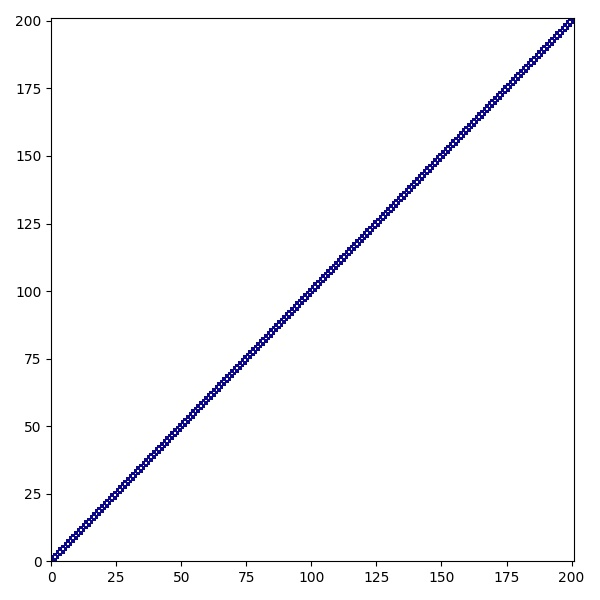
\includegraphics[width = 0.7\columnwidth]{graph.jpg}
\caption{Gráf szomszédossági mátrixa}
\end{figure}
\subsection{Részgráf}
Irányítatlan élekből álló út, az első és az utolsó csúcson hurokéllel.
\begin{figure}[H]
\centering
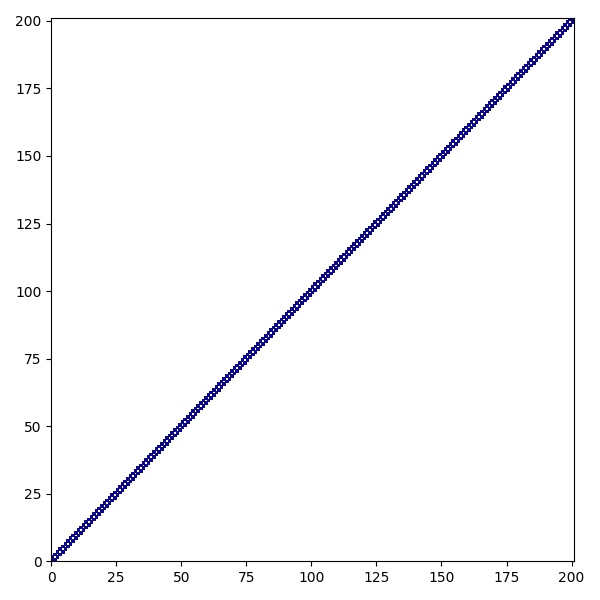
\includegraphics[width = 0.7\columnwidth]{subgraph_00.jpg}
\caption{0. részgráf szomszédossági mátrixa}
\end{figure}
\section{Szimulációk}
\subsection{Kvantum szimuláció}
Kezdőcsúcs: 100
Bolyongók: 1
Lépésszám: 100
\begin{figure}[H]
\centering
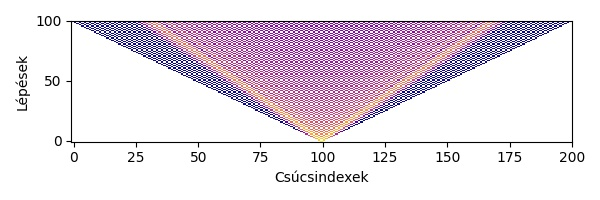
\includegraphics[width = 0.7\columnwidth]{sim00.jpg}
\caption{0. szimuláció}
\end{figure}
\end{document}